\chapter{Metode}\label{sec:metode}
\section{Model gibanja}\label{sec:model-gibanja}
% Ponovi teorijo energijske porabe in kako pridemo do gibanja
% Dokazi, da lahko gibanje opazujemo s kamerami
% Teorija, da je najboljši približek optični tok
Da mišice lahko s svojimi kontrakcijami spravijo telo v pogon, potrebujejo energijo, pri tem pa se del energije pretvarja v toploto, ki ji pravimo energijska poraba \cite{scott2005misconceptions}. Energijska poraba nastaja zaradi gibanja telesa, zato jo lahko določimo z opazovanjem kinematike \cite{levine2005measurement}. Zaradi omejitev kontaktnih senzorjev in slabih lastnosti srčnega utripa so v študijah, ki so opisane v poglavju \ref{sec:podobna-dela}, dokazali, da lahko z opazovanjem kinematike z računalniškim vidom določimo energijsko porabo. 

Naj bo delec z maso $m$ predstavljen kot točka prizora $\vec{p} = [X~Y~Z]^\top$, na sliki \ref{fig:model-gibanja}. $X$, $Y$ in $Z$ predstavljajo koordinate na posameznih oseh v koordinatnem sistemu kamere \cite{trucco1998introductory}. Gibanje delca $\vec{p}$ lahko predstavimo z vektorjem hitrosti $\vec{v} = [v_X~v_Y~v_Z]^\top$, $\vec{v} \in \mathcal{V} \subset \mathbb{R}^3$, kjer so $v_X$, $v_Y$ in $v_Z$ hitrosti glede na osi in $\mathcal{V}$ vektorski prostor. Kadar imamo v prostoru več masnih delcev, množico vektorjev hitrosti imenujemo \textbf{polje hitrosti} (angl. Velocity Field) $\mathbf{H}: \mathbb{R}^3 \to \mathcal{V}$, kjer velja $\vec{p} \mapsto \vec{v}$ \cite{trucco1998introductory}.


\begin{figure}
\centering
\begin{tikzpicture}%[tdplot_main_coords, scale=0.5]
[x={(0.8cm,0.4cm)}, y={(0cm,1cm)}, z={(0.8cm,-0.4cm)}, scale=0.5]
      
	% Coordinate system
    \coordinate (O) at (0,0,0);
    \coordinate (y) at (0,5,0);
    \coordinate (z) at (0,0,15);
    \coordinate (x) at (10,0,0);
    \draw [axis] (O) -- (y) node [above] {$y$};
    \draw [axis] (O) -- (z) node [below] {$z$};
    \draw [axis] (O) -- (x) node [below] {$x$};
    \node (izhodisce) [below] at (O) {$o$};
    
    % delec
    \coordinate (p) at (5,3,10);
    \draw [fill=black] (p) circle (1.5mm) node [below] {$\vec{p}$};
    \draw [dash] (O) -- (p);
    \draw [dash] (5,0,0) node [above] {$X$} -- (5,0,10);
    \draw [dash] (0,0,10) node [below] {$Z$} -- (5,0,10);
    \draw [dash] (5,0,10) -- (5,3,10);
    
    % hitrost
    \draw [velocity] (p) -- (6,4,10) node [above] {$\vec{v}$};
    

\end{tikzpicture}
\caption[Predstavitev delca $\vec{p}$ v koordinatnem sistemu kamere]{Predstavitev delca $\vec{p}$ v koordinatnem sistemu kamere. Delec je predstavljen kot točka prizora z vektorjem hitrosti $\vec{v}$ \cite{trucco1998introductory}.}
\label{fig:model-gibanja}
\end{figure}




Relativno gibanje delca $\vec{p}$ glede na koordinatno izhodišče kamere $O$ lahko opišemo kot:

\begin{equation}
	\vec{v} = -\vec{T}-\omega\times\vec{p},
\end{equation}

kjer je $\vec{T}$ translatorna hitrost in $\omega$ kotna hitrost \cite{trucco1998introductory}. Po komponentah lahko gibanje opišemo z enačbo \eqref{eq:gibanje}

\begin{equation} \label{eq:gibanje}
	\begin{bmatrix}
	v_X \\ v_Y \\ v_Z
	\end{bmatrix}
    =
    \begin{bmatrix}
    - T_X - \omega_Y Z + \omega_Z Y \\
    - T_Y - \omega_Z X + \omega_X Z \\
    - T_Z - \omega_X Y + \omega_Y X
    \end{bmatrix}.
\end{equation}

Gibanje telesa v prostoru torej lahko opišemo s poljem hitrosti $\vec{H}$.










\section{Optični tok} \label{sec:opticni-tok}
% Teorija optičnega toka
% vrste optičnega toka
% Kateri tip smo mi uporabili
% Zakaj smo tega uporabili
% Kako smo ga uporabili
% Problemi naše predpostavke
% Rešitev s kalibracijo velikosti
Za namen razlage upoštevamo perpektivni model kamere, kjer je \cite{trucco1998introductory}:

\begin{itemize}
\item \textbf{optična os} enaka $Z$ osi koordinatnega sistema kamere.
\item \textbf{Gibajoči masni delec} je predstavljen enako kot v poglavju \ref{sec:model-gibanja}.
\item \textbf{Osvetlitev} se ne spreminja.
\end{itemize}

Sliko delca $\vec{q} = [x~y]^\top$ na slikovni ravnini $\mathit{\Omega} \subset \mathbb{R}^2$, kjer sta $x$ in $y$ slikovni koordinati, lahko predstavimo z enačbo

\begin{equation}\label{eq:slika-delca}
	\vec{q} = f \frac{\vec{p}}{Z},
\end{equation}

kjer je $f$ goriščna razdalja kamere \cite{trucco1998introductory}. Delec in njegova slika sta predstavljena na sliki \ref{fig:optical-flow} S časovnim odvodom enačbe \eqref{eq:slika-delca}, dobimo hitrost delca na slikovni ravnini:

\begin{equation}\label{eq:hitrost-slike-delca}
	\vec{u} = f \frac{Z\vec{v}-v_Z\vec{p}}{Z^2},
\end{equation}

kjer je $\vec{u} \in \mathcal{U} \subset \mathbb{R}^2$.




\begin{figure}
\centering
\begin{tikzpicture}%[tdplot_main_coords, scale=0.5]
[x={(0.8cm,0.4cm)}, y={(0cm,1cm)}, z={(0.8cm,-0.4cm)}, scale=0.5]

	% Coordinate system
    \coordinate (O) at (0,0,0);
    \coordinate (oo) at (0,0,5);
    \coordinate (y) at (0,5,0);
    \coordinate (z) at (0,0,15);
    \coordinate (x) at (10,0,0);
    \draw [axis] (O) -- (y) node [above] {$y$};
    \draw [base-axis] (O) -- (oo);
    \draw [axis] (O) -- (x) node [below] {$x$};
    \node (izhodisce) [below] at (O) {$o$};
    
    % Image plane
    \coordinate (ol) at (-5,0,5);
    \coordinate (or) at (5,0,5);
    \coordinate (ot) at (0,3,5);
    \coordinate (ob) at (0,-3,5);
    \coordinate (lb) at (-5,-3,5);
    \coordinate (rb) at (5,-3,5);
    \coordinate (lt) at (-5,3,5);
    \coordinate (rt) at (5,3,5);
    \draw [plane] (lb) -- (lt) -- (rt) -- (rb) -- cycle;
    \draw [dash] (ol) -- (or);
    \draw [dash] (ob) -- (ot);
    \node [xshift=3mm, yshift=5mm] at (lb) {$\mathit{\Omega}$};
    % Draw the rest of axis
    \draw [axis] (oo) -- (z) node [below] {$z$};
    
    % focal length
    \coordinate (of) at (-5,0,0);
   	\draw [dash] (O) -- (of);
    \draw [<->] (of) -- (ol) node [below] at (-5,0,2.5) {$f$};
    
    % delec
    \coordinate (p) at (5,3,10);
    \draw [fill=black] (p) circle (1.5mm) node [below] {$\vec{p}$};
    \draw [dash, name path=line 1] (O) -- (p);
    \draw [dash] (5,0,0) node [above] {$X$} -- (5,0,10);
    \draw [dash] (0,0,10) node [below] {$Z$} -- (5,0,10);
    \draw [dash] (5,0,10) -- (p);
    
    % hitrost
    \coordinate (v) at (6,4,10);
    \draw [velocity] (p) -- (v) node [above] {$\vec{v}$};
    \draw [dash] (O) -- (v);
    
    % slika delca
    \coordinate (q) at (2.5,1.5,5);
    \draw [fill=black] (q) circle (1mm) node [below] {$\vec{q}$};
    \draw [dash] (2.5,0,5) node [below] {$x$} -- (q);
    \draw [dash] (0,1.5,5) node [left] {$y$} -- (q);
    
    %hitrost
    \draw [velocity] (q) -- (3,2,5) node [above] {$\vec{u}$};

\end{tikzpicture}
\caption[Preslikava hitrosti delca na slikovno ravnino $\mathit{\Omega}$]{ Preslikava hitrosti delca na slikovno ravnino $\mathit{\Omega}$. Gibajoči delec $\vec{p}$ ima sliko $\vec{q}$. Hitrost delca $\vec{v}$ ima sliko hitrosti $\vec{u}$, ki predstavlja idealni vektor gibanja. Koordinatni sistem predstavlja sistem kamere.}
\label{fig:optical-flow}
\end{figure}




Razširjena oblika enačbe \eqref{eq:hitrost-slike-delca}, kjer upoštevamo \eqref{eq:gibanje}, je zapisana z enačbo \eqref{eq:hitrost-slike-delca-raz} \cite{trucco1998introductory}. Prvi člen v posamezni enačbi predstavlja \textbf{translatorni del}, ostali členi pa sodijo v \textbf{rotacijski del}.

\begin{equation}\label{eq:hitrost-slike-delca-raz}
\begin{aligned}
	u_x = & \frac{T_Z x - T_X f}{Z} - \omega_Y f + \omega_Z y + \frac{\omega_X x y}{f} - \frac{\omega_Y x^2}{f} \\
    u_y = & \frac{T_Z y - T_Y f}{Z} - \omega_X f + \omega_Z x + \frac{\omega_Y x y}{f} - \frac{\omega_X y^2}{f}
\end{aligned}
\end{equation}

Kadar imamo na slikovni ravnini več slik delcev, množico vektorjev hitrosti $\vec{u}$ imenujemo \textbf{polje gibanja} (angl. Motion Field) $\vec{G} : \mathit{\Omega} \to \mathcal{U}$, kjer velja $ \vec{q} \mapsto \vec{u}$ \cite{trucco1998introductory}. Polje gibanja $\vec{G}$ lahko razumemo kot projekcijo polja hitrosti $\vec{H}$ na slikovno ravnino, zato ta predstavlja idealno rekonstrukcijo gibanja. V praksi do polja gibanja ne moremo dostopati, zato se poslužujemo njegovih približkov.  

Video posnetek je sestavljen iz sekvence slik, to pa lahko opišemo kot funkcijo osvetljenosti slikovnega elementa $I(\vec{x},t)$, na poziciji $\vec{x} = [x~y]^\top$ ob času $t$ \cite{wedel2011stereo}. Gibanje oseb opazimo kot premikanje pikslov skozi čas, pri čemer predpostavimo, da osvetljenost posameznega piklsa ostaja konstantnta \cite{trucco1998introductory}. Stacionarnost osvetljenosti slikovnega elementa lahko opišemo z enačbo  

\begin{equation}
	\frac{d I(\vec{x}, t)}{dt} = \frac{\partial I}{\partial x} \frac{dx}{dt} + \frac{\partial I}{\partial y} \frac{dy}{dt} + \frac{\partial I}{\partial t} = 0,
\end{equation}

to pa lahko zapišemo z vektorjem hitrosti slikovnega elementa $\vec{w} \in \mathcal{W} \subset \mathbb{R}^2$ v kompaktnejšo obliko

\begin{equation}\label{eq:opticni-tok}
	(\nabla I)^\top \vec{w} + I_t = 0.
\end{equation}

Enačba \eqref{eq:opticni-tok} predstavlja \textbf{omejitev optičnega toka} \cite{trucco1998introductory}. Če v enačbi \eqref{eq:opticni-tok} normaliziramo prostorski gradient $(\nabla I)$, v enačbi \eqref{eq:aperture-problem} opazimo, da lahko  določimo le hitrost, ki je vzporedna prostorskemu gradientu. Pojav je znan kot problem reže (angl. Aperture problem) \cite{trucco1998introductory}. 

\begin{equation}\label{eq:aperture-problem}
	\frac{(\nabla I)^\top \vec{w}}{\| \nabla I \|} = - \frac{I_t}{\| \nabla I \|} = w_n
\end{equation}

\textbf{Problem reže} si lahko razlagamo na način opazovanja gibanja daljice na beli podlagi skozi režo tako, da ne vidimo koncev. Zaradi omejene vizualne informacije lahko določimo hitrost le v pravokotni smeri na daljico \cite{trucco1998introductory}. Razlaga je predstavljena na sliki \ref{fig:aperture-problem}.




\begin{figure}[htb]
\centering
\begin{tikzpicture}[scale=0.7]
\tikzset{aperture/.style = {
fill=teal!50, 
draw=teal!50!black!80
}}
\tikzset{stick/.style = {
fill=orange!50!black!50, 
draw=orange!50!black!80, solid, thick,
minimum width = 1mm, minimum height=7cm
}}
  \begin{scope}
  		\coordinate (top) at (10,10);
        \coordinate (bottom) at (0,0);
       	\coordinate (center) at (5,5);

  		% palica
        \coordinate (pc) at (4,4);
        \path (pc) node[stick,rotate = 45]{};
        \draw [fill] (pc) circle (0.5mm);
        \coordinate (pc2) at (6,4);
        \path (pc2) node[stick, rotate = 45, dashed, fill=none]{};
        \draw [fill] (pc2) circle (0.5mm);
        
        % vektor
        \draw [velocity, draw=black] (pc) -- ++(1,1) node [below] {${\vec{w}_n}$};
        \draw [velocity, draw=black] (pc) -- (pc2) node [below] {$\vec{w}$};
  		% aperture	
		\draw [aperture, opacity=0.8] (bottom) rectangle (top) (center) circle (20mm);  
  \end{scope}


\end{tikzpicture}
\caption[Problem reže]{Problem reže. Ker skozi režo ne vidim koncev daljice, lahko določimo le hitrost v pravokotni smeri na daljico \cite{trucco1998introductory}.}
\label{fig:aperture-problem}
\end{figure}




Kadar imamo na slikovni ravnini več premikajočih slikovnih elementov, vektorsko polje hitrosti $\vec{w}$ imenujemo \textbf{optični tok} (angl. Optical flow) $\vec{O}: \mathit{\Omega} \to \mathcal{W}$, kjer velja $ \vec{q} \mapsto \vec{w}$ \cite{trucco1998introductory}. Optični tok je dobra aproksimacija polja gibanja v točkah visokega prostorskega gradienta svetlosti in konstantne osvetlitve.



\subsection{Metode estimacije optičnega toka}\label{sec:metode-of}

Metode estimacije optičnega toka $\vec{O}$ v grobem delimo na diferencialne in {ujemalne} metode \cite{trucco1998introductory}. Z \textbf{diferencialnimi metodami} računamo optični tok z uporabo parcialnih diferencialnih enačb ali minimizacijskimi metodami. Z metodami dobimo \textbf{gost optični tok}, kar pomeni, da je optični tok določen za vsak slikovni element \cite{trucco1998introductory}. Te metode zelo natačno opisujejo optični tok in ne proizvajajo vrednosti, ki lokalno odstopajo, zato je optični tok gladek \cite{brox2011large}.  Glavni problem teh metod je, da so računsko zelo zahtevne \cite{trucco1998introductory}.

Pri \textbf{ujemalnih metodah} računamo optični tok le na značilnih točkah \cite{trucco1998introductory}. Zaradi uporabe značilk so te metode lahko bolj efektivne, saj ne potrebujemo določevanja korespondenc za vse piksle. Prav tako se lahko uporabijo za računanje optičnega toka v realnem času, saj niso računsko zahtevne. Po \cite{trucco1998introductory} je največja težava teh metod, da računajo \textbf{redek optični tok}, saj je ta določen le za slikovne elemete, ki predstavljajo značilne točke. Prav tako delujejo dobro le pri majhnih premikih, ker temeljijo na Taylorjevi aproksimaciji enačbe \eqref{eq:opticni-tok} \cite{wedel2011stereo}. 

V nadaljevanju predstavljamo diferencialno metodo Farneb{\"a}ck algoritem.

\subsubsection{Farneb{\"a}ck algoritem.}
Alogritem temelji na estimaciji premika z razčlenjevanjem polinoma  po enačbi \eqref{eq:polinom}, kjer je $\vec{A}$ simetrična matrika, $\vec{b}$ vektor in $c$ skalar \cite{farneback2003two}.

\begin{equation}\label{eq:polinom}
	f(\vec{x}) \sim \vec{x}^\top \vec{A} \vec{x} + \vec{b}^\top \vec{x} + c
\end{equation}

Ideja temelji na tem, da aproksimiramo okolico piksla s kvadratičnim polinomom, pri čemer želimo najti premik piksla na poziciji $\vec{x}$ z minimizacijo enačbe \eqref{eq:polinom-min} in omejitvijo \eqref{eq:omejitev-polinoma}. $\vec{A}_1(\vec{x})$ in $\vec{b}_1(\vec{x})$ sta razčlenitvena koeficienta za prvo sliko, $\vec{A}_2(\vec{x})$ in $\vec{b}_2(\vec{x})$ koeficienta za drugo sliko in $w(\Delta\vec{x})$ je utežna funkcija za sosedne točke.

\begin{align}
\vec{A}(\vec{x}) = & \frac{\vec{A}_1(\vec{x} + \vec{A}_2(\vec{x}))}{2} \\
\Delta\vec{b}(\vec{x}) = & - \frac{1}{2}\left(\vec{b}_2(\vec{x}) - \vec{b}_1(\vec{x})\right) 
\end{align}

\begin{equation}\label{eq:polinom-min}
\sum_{\Delta x \in I} w(\Delta\vec{x}) \| \vec{A}(\vec{x} + \Delta\vec{x})\vec{d}(\vec{x}) - \Delta\vec{b}(\vec{x} +\Delta\vec{x}) \|^2
\end{equation}

\begin{equation}\label{eq:omejitev-polinoma}
\vec{A}(\vec{x})\vec{d}(\vec{x}) = \Delta\vec{b}(\vec{x})
\end{equation}

Rešitev minimizacije enačbe \eqref{eq:polinom-min} je enačba \eqref{eq:polinom-resitev}

\begin{equation}\label{eq:polinom-resitev}
 \vec{d}(\vec{x}) = \left( \sum w \vec{A}^\top \vec{a} \right)^{-1} \sum w \vec{A}^\top \Delta\vec{b}
\end{equation}

Evaluacija algoritma je bila narejena v \cite{Geiger2012CVPR}. Rezultati so povzeti v tabeli \ref{tab:farneback}. Algoritem so preverjali s procesorjem z 1 jedrom \@ \SI{2.5}{GHz}.

\begin{table}
	\centering
    \begin{tabular}{S[table-format=2.2] S[table-format=2.2] S[table-format=2.1] S[table-format=2.1] S[table-format=3.2] S[table-format=1]}
    \toprule
    \multicolumn{1}{c}{\textbf{Out-Noc}} & \multicolumn{1}{c}{\textbf{Out-All}} & \multicolumn{1}{c}{\textbf{Avg-Noc}} & \multicolumn{1}{c}{\textbf{Avg-All}} & \multicolumn{1}{c}{\textbf{Gostota}} & \multicolumn{1}{c}{\textbf{Čas izvajanja}} \\
    \midrule
    47.59~\% & 54.00~\% & 17.3~px & 25.3~px & 100.00~\% & 1~s\\
    \bottomrule
    \end{tabular}
    \caption[Evaluacija Farneb{\"a}ck algoritma v KITTI Vision Benchmark 2012]{Evaluacija Farneb{\"a}ck algoritma v KITTI Vision Benchmark 2012 \cite{Geiger2012CVPR}. Metrika Out-Noc predstavlja procent pikslov, ki težijo k napakam v območju, kjer ni prekrivnosti. Out-all je procent pikslov, ki težijo k napakam v celoti. Avg-Noc je povprečna napaka disparitete v območjih neprekrivnsoti. Avg-All je povprečna napaka disparitete v celoti. Gostota predstavlja procent pikslov, za katere je metoda določila referenco \cite{Geiger2012CVPR}.}
    \label{tab:farneback}
\end{table}




\section{Prostorski tok}
% Teorija prostorskega toka
% Katero metodo smo mi uporabili in zakaj
Optični tok $\vec{O}$ predstavlja aproksimacijo polja gibanja $\vec{G}$, ta pa je projekcija polja hitrosti $\vec{H}$ na slikovno ravnino $\mathit{\Omega}$ \cite{trucco1998introductory}. Če pogledamo z druge perspektive, ni optični tok $\vec{O}$ nič drugega kot projekcija aproksimacije polja hitrosti $\vec{H}$, ki jo po analogiji lahko imenujemo \textbf{prostorski tok} (angl. Scene Flow) \cite{vedula1999three}. 

Za namen razlage upoštevamo enake omejitve kamere, masnega delca in osvetlitve, kot v poglavju \ref{sec:opticni-tok}. Predpostavimo, da imamo v prostoru površino $f(x,y,z) = 0$ na kateri imamo gibajoč točkovni delec $\vec{p} = \vec{p}(t)$. Na slikovni ravnini $\mathit{\Omega}$ imamo njegovo sliko $\vec{q}$ \cite{vedula1999three}. Vizualni prikaz prizora lahko vidimo na sliki \ref{fig:scene-flow}. 




\begin{figure}
\centering
\begin{tikzpicture}%[tdplot_main_coords, scale=0.5]
[x={(0.8cm,0.4cm)}, y={(0cm,1cm)}, z={(0.8cm,-0.4cm)}, scale=0.5]

	% Coordinate system
    \coordinate (O) at (0,0,0);
    \coordinate (oo) at (0,0,5);
    \coordinate (y) at (0,5,0);
    \coordinate (z) at (0,0,15);
    \coordinate (x) at (10,0,0);
    \draw [axis] (O) -- (y) node [above] {$y$};
    \draw [base-axis] (O) -- (oo);
    \draw [axis] (O) -- (x) node [below] {$x$};
    \node (izhodisce) [below] at (O) {$o$};
    
    % Image plane
    \coordinate (ol) at (-5,0,5);
    \coordinate (or) at (5,0,5);
    \coordinate (ot) at (0,3,5);
    \coordinate (ob) at (0,-3,5);
    \coordinate (lb) at (-5,-3,5);
    \coordinate (rb) at (5,-3,5);
    \coordinate (lt) at (-5,3,5);
    \coordinate (rt) at (5,3,5);
    \draw [plane] (lb) -- (lt) -- (rt) -- (rb) -- cycle;
    \draw [dash] (ol) -- (or);
    \draw [dash] (ob) -- (ot);
    \node [xshift=3mm, yshift=5mm] at (lb) {$\mathit{\Omega}$};
    % Draw the rest of axis
    \draw [axis] (oo) -- (z) node [below] {$z$};
    
    % focal length
    \coordinate (of) at (-5,0,0);
   	\draw [dash] (O) -- (of);
    \draw [<->] (of) -- (ol) node [below] at (-5,0,2.5) {$f$};
    
    % povrsina
    \begin{scope}
    \coordinate (p0) at (3,1,12);
    \coordinate (p1) at (3,5,12);
    \coordinate (p2) at (7,5,12);
    \coordinate (p3) at (7,1,12);
   
    \draw [plane, fill=purple!20, draw=purple!50!black!50,] 
    			   (p0) .. controls (3,4,10) .. (p2)
                        .. controls (7,3,10) .. (p3) 
                        .. controls (5,1,10) .. cycle;
    \node at (6,2,12) {$f$};
    \end{scope}
    
    
    
    % delec
    \coordinate (p) at (5,3,10);
    \draw [fill=black] (p) circle (1.5mm) node [below] {$\vec{p}$};
    \draw [dash, name path=line 1] (O) -- (p);
    %\draw [dash] (5,0,0) node [above] {$X$} -- (5,0,10);
    %\draw [dash] (0,0,10) node [below] {$Z$} -- (5,0,10);
    %\draw [dash] (5,0,10) -- (p);
    
    % hitrost
    \coordinate (v) at (6,4,10);
    \draw [velocity] (p) -- (v) node [above] {$\vec{\mu}$};
    \draw [dash] (O) -- (v);
    
    % slika delca
    \coordinate (q) at (2.5,1.5,5);
    \draw [fill=black] (q) circle (1mm) node [below] {$\vec{q}$};
    \draw [dash] (2.5,0,5) node [below] {$x$} -- (q);
    \draw [dash] (0,1.5,5) node [left] {$y$} -- (q);
    
    %hitrost
    \draw [velocity] (q) -- (3,2,5) node [above] {$\vec{w}$};
\end{tikzpicture}
\caption[Vizualni prikaz vektorja prostorskega toka $\vec{w}$]{Vizualni prikaz vektorja prostorskega toka $\vec{w}$. V prostoru imamo površino $f$ na kateri leži gibajoči točkovni delec $\vec{p}$ \cite{vedula1999three}. Na slikovni ravnini $\mathit{\Omega}$ imamo sliko delca $\vec{q}$ s prostorskim tokom $\vec{w}$.}
\label{fig:scene-flow}
\end{figure}



Ker je slika projekcija delca na slikovno ravnino $\mathit{\Omega}$, lahko zapišemo $\vec{q} = \vec{q}(\vec{p})$. Hitrost slike določimo po enačbi \eqref{eq:opticni-tok-sf}, ki predstavlja enačbo vektorja optičnega toka $\vec{w}$, kot projekcijo prostorskega toka \cite{vedula1999three}. 


\begin{equation}\label{eq:opticni-tok-sf}
	\vec{w} = \frac{d\vec{q}}{dt} = \frac{\partial \vec{q}}{\partial \vec{p}}\frac{d\vec{p}}{dt}
\end{equation}

Če predpostavimo, da imamo dovoj informacije o sistemu, da lahko določimo inverzno funkcijo $\vec{p} = \vec{p}(\vec{q},t)$, kjer je masni delec $\vec{p}$ projekcija slike $\vec{q}$, lahko določimo njegovo hitrost $\vec{\mu} \in \mathcal{\Mu} \subset \mathbb{R}^3$ z enačbo \eqref{eq:scene-flow}. Slednja je sestavljena iz dveh delov. Prvi člen je projekcija vektorja optičnega toka $\vec{w}$ na tangentno ravnino površine $f$, v točki, kjer se nahaja delec $\vec{p}$ \cite{vedula1999three}. Drugi člen je hitrost spreminjanja oddaljenosti delca od slikovne ravnine $\mathit{\Omega}$, ko slika delca stoji na miru. 

\begin{equation}\label{eq:scene-flow}
	\vec{\mu} = \frac{d\vec{p}}{dt} = \frac{\partial \vec{p}}{\partial \vec{q}} \frac{d\vec{q}}{dt} + \left.\frac{\partial \vec{p}}{\partial t}\right|_\vec{q}
\end{equation}

Kadar imamo v prostoru več, med seboj neodvisnih premikajočih masnih delcev, vektorsko polje hitrosti $\vec{\mu}$ imenujemo prostorski tok (angl. Scene Flow) $\vec{S}: \mathcal{W} \times \mathbb{R} \to \mathcal{\Mu}$, kjer velja $(\vec{w}, \dot{Z}) \mapsto \vec{\mu}$ \cite{yan2016scene}. $\dot{Z}$ predstavlja hitrost spreminjanja globine.

\subsection{Metode estimacije prostorskega toka}
Konvencionalne metode estimacije prostorskega toka so se razvile iz optičnega toka, in dodatne informacije o globini \cite{yan2016scene}. Slednjo lahko pridobimo s parom stereo kamer ali z uporabo sistemov večih kamer \cite{jaimez2015primal}. Vektor hitrosti prostorskega toka lahko v takih sistemih aproksimiramo z $\vec{\mu} = \left[w_x~w_y~\dot{d}\right]^\top$, kjer sta $(w_x, w_y)$ komponenti vektorja optičnega toka $\vec{w}$, $\dot{d}$ pa časovna sprememba disparitete \cite{yan2016scene}.

Z razvojem RGB-D kamer, kjer RGB predstavlja barvno sliko, D pa globinsko sliko, smo dobili cenovno dostopne in natančne sisteme, ki omogočajo implementacijo hitrih algoritmov prostorskega toka \cite{yan2016scene,jaimez2015primal}. Ti večinoma temeljijo na globalni variacijski metodi, kjer rešujemo minimizacijski problem 

\begin{equation}\label{eq:minimizacijski-problem}
	\min_{\mu}\{E_D(\vec{\mu}) + E_R(\vec{\mu})\}
\end{equation}

V podatkovnem delu funkcionala \eqref{eq:minimizacijski-problem} $E_D(\vec{\mu})$ \eqref{eq:podatkovni-del} upoštevamo konstantno osvetljenost \eqref{eq:konstantna-osvetljenost} in konsistentnost spreminjana globine \eqref{eq:konsistentnost-globine}, kjer je  $\Psi$ cenilka. Ponavadi je uporabljena $L_2$ norma $\Psi(x) = \| x \|^2$ \cite{yan2016scene}. $\alpha$ v \eqref{eq:podatkovni-del} predstavlja utež.

\begin{equation}\label{eq:konstantna-osvetljenost}
	E_{KO} = \sum_\Omega \Psi( I(\vec{q} + \vec{w}) - I(\vec{q}))
\end{equation}

\begin{equation}\label{eq:konsistentnost-globine}
	E_{KG} = \sum_\Omega \Psi\left( Z(\vec{q} + \Delta \vec{q}) - Z(\vec{q}) - \dot{Z}(\vec{q}))\right)
\end{equation}

\begin{equation}\label{eq:podatkovni-del}
	E_D = E_{KO} + \alpha E_{KG}
\end{equation}

V regularizacijskem delu funkcionala \eqref{eq:minimizacijski-problem} $E_R(\vec{\mu})$ pa uporabimo enačbo \eqref{eq:regularizacijski-del}

\begin{equation}\label{eq:regularizacijski-del}
	E_R = \sum_\Omega \Psi\left( \nabla w_x \right) + \Psi\left( \nabla w_y \right) + \Psi\left( \nabla \dot{Z} \right)
\end{equation}

V nadaljevanju predstavljamo globalno variacijsko metodo PD-Flow algoritem.


\subsubsection{PD-Flow algoritem.}\label{sec:pd-flow}
Algoritem spada pod globalne variacijske metode \cite{jaimez2015primal}. Za cenilko $\Psi$ v \eqref{eq:konstantna-osvetljenost} in \eqref{eq:konsistentnost-globine} avtorji uporabljajo $L_1$ normo. Za utež $\alpha$ v podatkovnem delu funkcionala \eqref{eq:podatkovni-del} se v tem algorimu uporablja funkcija 

\begin{equation}\label{eq:utez}
 \alpha(x,y) = \frac{\mu_0}{1 + k_\mu \left( \frac{\partial Z^2}{\partial x} + \frac{\partial Z^2}{\partial y} + \frac{\partial Z^2}{\partial t} \right)},
\end{equation}

kjer sta empirično določena parametra $\mu_0 = 75$ in $k_mu = 1000$. Za izračun podatkovnega dela uporabljajo hierarhično metodo grajenja slikovne piramide, pri tem pa uporabljajo linearizacijo podatkovnega dela \eqref{eq:podatkovni-del} \cite{jaimez2015primal}.

Jaimez et al. v delu \cite{jaimez2015primal} predstavi nov regularizacijski del \eqref{eq:regularizacijski-del-pdflow}, kjer upošteva še geometrijo prizora s faktorjem $\vec{r}$ \eqref{eq:faktor-prizora}. Z njim upošteva, da lahko sosednji slikovni elementi predstavljajo točke v prostoru, ki so si različno oddaljene.

\begin{equation}\label{eq:regularizacijski-del-pdflow}
E_R = \sum_\Omega \Psi\left( (\nabla w_x)^\top \vec{r} \right) + \Psi\left( (\nabla w_y)^\top \vec{r} \right) + \Psi\left( (\nabla \dot{Z})^\top \vec{r} \right)
\end{equation}

\begin{equation}\label{eq:faktor-prizora}
\vec{r} =
\begin{bmatrix}
\frac{1}{\sqrt{\frac{\partial X^2}{\partial x} + \frac{\partial Z^2}{\partial x}}} &
\frac{1}{\sqrt{\frac{\partial Y^2}{\partial y} + \frac{\partial Z^2}{\partial y}}}
\end{bmatrix}^\top
\end{equation}

Evaluacija PD-Flow algoritma je prikazana v tabeli \ref{tab:pdflow}. V tabeli so zapisani še rezultati RGB-D flow algoritma, ki za cenilko $\Psi$ ravno tako uporablja $L_1$ normo \cite{jaimez2015primal}. Opazimo lahko, da se PD-Flow po metrikah bolje odnese. Največji izboljšanje vidimo pri času izvajanja algoritma.

\begin{table}
	\centering
    \begin{tabular}{l S[table-format=1.3] S[table-format=2.3] S[table-format=3.3] S[table-format=3.3]}
    \toprule
    \textbf{Algoritem} & \multicolumn{1}{c}{\textbf{NRMS-V}} & \multicolumn{1}{c}{\textbf{AAE}} & \multicolumn{1}{c}{\textbf{Čas izvajanja [s]}} & \multicolumn{1}{c}{\textbf{MAX-V [m]}} \\
    \midrule
    \textbf{PD-Flow} & \boldentry{1.3}{0.068} & \boldentry{2.3}{6.653} & \boldentry{3.3}{7.150} & 0.111 \\
    RGB-D flow & 0.096 & 15.58 & 119.1 & 0.111 \\
    \bottomrule
    \end{tabular}
    \caption[Evaluacija PD-Flow algoritma]{Evaluacija PD-Flow algoritma in primerjava z algoritmom RGB-D flow, ki uporablja enako cenilko $\Psi$ \cite{jaimez2015primal}. Za metrike se uporabljata povprečna kotna napaka (AAE) in normaliziran koren srednje kvadratične napake magnitude hitrosti (NRMS-V), kjer se največja magnituda (MAX-V) uporablja za normalizacijo \cite{jaimez2015primal}. Opazimo lahko, da se PD-Flow po metrikah bolje odnese. Največji izboljšanje vidimo pri času izvajanja algoritma. Odebeljene vrednosti predstavljajo najboljšo vrednost.}
    \label{tab:pdflow}
\end{table}









\section{Deskriptorji}
% Težave optičnega toka in prostorskega toka.
% Kako bi te težave rešili z deskriptorji
% Našli specifične deskriptorje
Klasične metode optičnega toka so občutljive na šum, diskontinuitete gibanja ter spremembe v osvetljenosti objekta~\cite{brox2011large}, pri novejših pa še vedno obstaja problem pravilne ocene amplitude gibanja zaradi \textbf{pojava paralakse}~\cite{xu2012scale} -- objekti, ki so bolj oddaljeni od kamere imajo manjšo jakost optičnega toka. 


Ker je prostorski tok projekcija optičnega toka v prostor ima podobne probleme kot optični tok \cite{yan2016scene}. Večja natančnost algoritma zahteva večjo \textbf{računsko zahtevnost}, kar vodi v manjšo učinkovitost. \textbf{Okluzija}, ki se lahko pogostokrat pojavi, krši konsistentnost podatkov skozi čas, in lahko vodi v napačno določitev korespondenc \cite{yan2016scene}. Pri \textbf{hitrem gibanju} večina algoritmov ne deluje, saj temeljijo na predpostavki kratkih premikov na časovno enoto. Zaradi \textbf{sprememb osvetlitve} prizora postane estimacija prostorskega toka neuporabna \cite{yan2016scene}. Prav tako lahko pride do problemov, ko imamo \textbf{pomanjkanje teksture}, saj težje izračunamo gradient.

Surova optični in prostorski tok zaradi vrste problemov nista primerna za opis gibanja, čeprav predstavljata najbolj naravno metodo estimacije energijske porabe. Tudi če zagotovimo idealno okolje (kontinuiteta gibanja, konstantna osvetljenost, počasno gibanje in dobra tekstura) imamo še vedno problem šuma zaradi CCD senzorja \cite{wedel2011stereo}. Ravno tako se ne moremo znebiti paralakse ali zagotoviti neodvisnosti od smeri po $X$ osi koordinatnega sistema kamere \cite{chaudhry2009histograms}. Pri tem moramo tudi opozoriti, da se število slikovnih elementov, ki predstavljajo merjenca, spreminja skozi čas. Vsa dejstva stremijo k temu, da moramo za pravilno merjenje energijske porabe uporabiti deskriptorje, ki izboljšajo robustnost optičnega in prostorskega toka \cite{chaudhry2009histograms}. 







\subsection{Histogrami orientiranega optičnega toka}\label{sec:hoof}
% Teorija teh deskriptorjev
% Kako smo jih mi uporabili
% Težave teh deskriptorjev
% Dodali nove deskriptorje
Ko se človek premika se optični tok temporalno spreminja. Lahko rečemo, da se spreminja karakteristični profil optičnega toka \cite{chaudhry2009histograms}. Prva ideja za deskriptor bi bila distribucija optičnega toka. Ker pa se profil spreminja zaradi paralakse, potrebujemo deskriptor, ki je invarianten na skalo in smer gibanja \cite{chaudhry2009histograms}.

Chaudhry et al. \cite{chaudhry2009histograms} predlaga uporabo histogramov orientiranega optičnega toka (HOOF), kjer vsak vektor optičnega toka zložimo v stolpec, glede na njegov kot in ga utežimo z njegovo velikostjo.

Vektorju optičnega toka $\vec{w} = [x~y]^\top$ določimo smer \eqref{eq:smer} in amplitudo \eqref{eq:amplituda} \cite{chaudhry2009histograms}. Interval smeri $\Theta$ je določen z \eqref{eq:interval}. 

\begin{align}
	\Theta = & \tan^{-1}\left( \frac{y}{x} \right) \label{eq:smer} \\
    \| \vec{w} \| = & \sqrt{x^2 + y^2} \label{eq:amplituda}
\end{align}

\begin{equation}\label{eq:interval}
	-\frac{\pi}{2} + \pi \frac{b - 1}{N_{HOOF}} \leq \Theta < - \frac{\pi}{2} + \pi \frac{b}{N_{HOOF}}
\end{equation}

Interval smeri \eqref{eq:interval} pomeni, da vektorju $\vec{w}$ določimo stolpec $b$, za katerega velja $1 \leq b \leq N_{HOOF}$, pri čemer je $N_{HOOF}$ celotno število stolpcev histograma, na podlagi smeri $\Theta$ \cite{chaudhry2009histograms}. Pri tem moramo za smer $\Theta$ upoštevati najmanjši predznačen kot med vektorjem $\vec{w}$ in koordinatno osjo $x$ koordinatnega sistema slikovne ravnine $\mathit{\Omega}$. Z drugimi besedami, upoštevamo samo kote na intervalu \eqref{eq:interval-kot}, kote na intervalu \eqref{eq:interval-kot2} pa preslikamo na interval \eqref{eq:interval-kot}. Interval \eqref{eq:interval-kot} razdelimo na $N_{HOOF}$ podintervalov, ki predstavljajo stolpce histograma. 

\begin{equation}\label{eq:interval-kot}
	\left[-\frac{\pi}{2}, \frac{\pi}{2}\right]
\end{equation}

\begin{equation}\label{eq:interval-kot2}
	\left(\frac{\pi}{2},\frac{3\pi}{2}\right)
\end{equation}

Vsak vektor $\vec{w}$, ki leži v podintervalu ali stolpcu $b$ bo prispeval svojo velikost $\|\vec{w} \|$ k njegovi vsoti \cite{chaudhry2009histograms}. Dobljeni histogram še normaliziramo, tako da je njegova vsota enaka $1$.





\begin{figure}[htb]
\centering
\begin{tikzpicture}
% LAYERS
\pgfdeclarelayer{bg}
\pgfsetlayers{bg,main}

 % LENGTHS
\newcommand{\csl}{5}
\newcommand{\vl}{3}

\begin{pgfonlayer}{bg}
% Coordinate system
\begin{scope}
	\tikzset{vec/.append style = {
    	draw=teal!50!black!80,
        very thick
    }}
	\begin{polaraxis}[hoof plot style]
		\addplot[vec, domain=0:1](20,x);
        \coordinate (v1) at (20, 0.7);
        \addplot[vec, domain=0:1.5](-45,x);
        \coordinate (v2) at (-45, 1);
        \addplot[vec, domain=0:0.5](160,x);
        \coordinate (v3) at (160,0.2);
	\end{polaraxis}
\end{scope}

\begin{scope}[xshift=10cm, yshift=0pt]
	\draw (0,1) rectangle (1,2) node (h1) [midway] {$1$};
    \draw (0,2) rectangle (1,3) node (h2) [midway] {$2$};
    \draw (0,3) rectangle (1,4) node (h3) [midway] {$3$};
    \draw (0,4) rectangle (1,5) node (h4) [midway] {$4$};
    \draw (0,5) rectangle (1,6) node (h5) [midway] {$5$};
    \draw (0,6) rectangle (1,7) node (h6) [midway] {$6$};
    \node at (0,0) {HOOF stolpci};
\end{scope}
\end{pgfonlayer}

\tikzset{show/.style={
	->,
    >=stealth,
    very thick,
    line width=1mm,
    draw=red!50!black!50,
    shorten >=2mm
    }}
\draw [show] (v1) circle (1mm);
\draw [show] (v1) to[out=90, in=180] (h4);
\draw [show] (v2) circle (1mm);
\draw [show] (v2) to[out=60, in=180] (h2);
\draw [show] (v3) circle (1mm);
\draw [show] (v3) to[out=90, in=180] (h4);
\end{tikzpicture}
\caption[Prikaz določitve HOOF histograma glede na kot vektorja]{Prikaz določitve HOOF histograma glede na kot vektorja optičnega toka $\vec{u}$. Slika prikazuje določitev za $6$ stolpcev.}
\label{fig:hoof-histogram}
\end{figure}




Preslikava intervala \eqref{eq:interval-kot2} v interval \eqref{eq:interval-kot} omogoča neodvisnost histograma od leve ali desne smeri gibanja \cite{chaudhry2009histograms}. Če se subjekt premika v levo ali desno, bo histogram enak. Z normiranjem histograma dobimo invariantnost na skalo \cite{chaudhry2009histograms}. Če se subjekt premika daleč ali blizu kamere, bo histogram enak. Ker je vsak prispevek vektorja sorazmeren njegovi amplitudi, šumni vektorji nimajo vpliva na obliko histograma \cite{chaudhry2009histograms}. Posledično lahko določimo histogram za celotno sliko in zato ne potrebujemo segmentacije ali subtrakcije gibajoče osebe iz ozadja. 

Edini parameter, ki ga moramo določiti za HOOF značilke je število stolpcev histograma $N_{HOOF}$. Chaudry et al \cite{chaudhry2009histograms} pravi, da moramo za dobro delovanje določiti najmanj $30$ stolpcev. 










\subsection{Histogrami absolutnih tokovnih amplitud}\label{sec:hafa}
% Opis dodatnih deskriptorjev
% Kako uporabili nove deskriptorje
HOOF deskriptor modelira samo smer gibanja. Za modeliranje amplitude gibanja moramo uporabiti drug deskriptor. Idejo deskriptorja za modeliranje amplitude gibanja smo dobili v delu \cite{pers2010histograms}, kjer so avtorji za opis gibanja uporabili histograme optičnega toka (HOF). Gre za histograme v dveh dimenzijah, ki posebej kvantizirata amplitudo in smer optičnega toka v podregijah slike. 

Vektorju optičnega toka $\vec{w}$, ki je opredeljen v poglavju \ref{sec:hoof}, ima amplitudo določeno na intervalu \eqref{eq:interval-amp1}. 

\begin{equation}\label{eq:interval-amp1}
	[0, \infty)
\end{equation}


Interval \eqref{eq:interval-amp1} lahko kvantiziramo po enačbi \eqref{eq:interval-amp2}. Ta pomeni, da vektorju $\vec{w}$ določimo stolpec $b$, za katerega velja $1 \leq b \leq N_{HAFA}$, pri čemer je $N_{HAFA}$ celotno število stolpcev histograma na podlagi amplitude $\| \vec{w} \|$. S tako kvantizacijo omejimo zgornjo mejo intervala \eqref{eq:interval-amp1} na parameter histograma $N_{HAFA}$. Ko tak histogram normiramo, ga imenujemo histogram absolutnih tokovnih amplitud (HAFA). Določitev HAFA histograma je prikazan na sliki \ref{fig:hafa-histogram}.

\begin{equation}\label{eq:interval-amp2}
	\frac{b-1}{N_{HAFA}} \leq \| \vec{w} \| < \frac{b}{N_{HAFA}}
\end{equation}




\begin{figure}[htb]
\centering
\begin{tikzpicture}
% LAYERS
\pgfdeclarelayer{bg}
\pgfsetlayers{bg,main}

 % LENGTHS
\newcommand{\csl}{5}
\newcommand{\vl}{3}

\begin{pgfonlayer}{bg}
% Coordinate system
\begin{scope}
	\tikzset{vec/.append style = {
    	draw=teal!50!black!80,
        very thick
    }}
	\begin{polaraxis}[polar plot style]
		\addplot[vec, domain=0:1](20,x);
        \coordinate (v1) at (20, 0.7);
        \addplot[vec, domain=0:1.5](-45,x);
        \coordinate (v2) at (-45, 1);
        \addplot[vec, domain=0:0.5](160,x);
        \coordinate (v3) at (160,0.2);
	\end{polaraxis}
\end{scope}

\begin{scope}[xshift=10cm, yshift=0pt]
	\draw (0,1) rectangle (1,2) node (h1) [midway] {$ 0.5$};
    \draw (0,2) rectangle (1,3) node (h2) [midway] {$1$};
    \draw (0,3) rectangle (1,4) node (h3) [midway] {$1.5$};
    \node at (0,0) {HAFA stolpci};
\end{scope}
\end{pgfonlayer}

\tikzset{show/.style={
	->,
    >=stealth,
    very thick,
    line width=1mm,
    draw=red!50!black!50,
    shorten >=2mm
    }}
\draw [show] (v1) circle (1mm);
\draw [show] (v1) to[out=-90, in=180] (h2);
\draw [show] (v2) circle (1mm);
\draw [show] (v2) to[out=60, in=180] (h3);
\draw [show] (v3) circle (1mm);
\draw [show] (v3) to[out=-90, in=180] (h1);
\end{tikzpicture}

\caption[Prikaz določitve HAFA histograma glede na velikost vektorja]{Prikaz določitve HAFA histograma glede na velikost vektorja optičnega toka $\vec{u}$. Slika prikazuje določitev za $3$ stolpce.}
\label{fig:hafa-histogram}
\end{figure}


























\section{Matematični modeli}\label{sec:matematicni-modeli}
Metode strojnega učenja s podpornimi vektorji (SVM) se pogosto uporabljajo za klasifikacijo in regresijo \cite{chang2011a}. Njihova popularnost temelji na visoki uspešnosti generalizacije brez potrebe po predhodnem znanju \cite{chapelle1999support}. Njihova performanca delovanja ni odvisna od števila značilk, saj jih ponavadi uporabljamo v primerih ko ima vhodni prostor značilk $\mathcal{W}^n$ veliko moč $n$. Cilj teh metod je, da generiramo matematični model in ga uporabimo za predikcijo izhoda $y$ \cite{hsu2003practical}. 








\subsection{Linearno ločljiva učna množica}
Imamo učne vzorce $\{ \vec{x}_i, y_i \} \in \mathcal{U}_l$, kjer je $\vec{x}_i \in \mathcal{\Xi}_l \subset \mathbb{R}^n~\forall i = 1, \ldots, l$ vektor značilk oziroma deskriptor in $y_i \in \mathit{\Omega}_l \subset \mathbb{R}~\forall i = 1, \ldots, l$ oznake razredov objektov \cite{chapelle1999support}. Za poenostavitev privzamemo, da imamo samo dva razreda $y_i \in \{-1,1\}$. 

Pri postopku s podpornimi vektorji v splošnem iščemo koeficiente $\vec{w} \in \mathcal{W} \subset \mathbb{R}^m$ ločilnih mej ali \textbf{hiper-ravnin} in prag $b$, ki razmejujejo prostor $\mathbb{R}^n$ tako, da so enako oddaljene od vzorcev $\vec{x}$ iz različnih razredov $\mathcal{C}_i~\forall i= 1, \ldots, p$, kot je prikazano na sliki \ref{fig:svm-locljivo} \cite{chapelle1999support}. Pri tem velja omejitev

\begin{equation}\label{eq:omejitev-ravnine}
	y_i(\vec{w} \vec{x}_i + b) \geq 1, i=1, \ldots, l.
\end{equation}





\begin{figure}[htb]
\centering
\begin{tikzpicture}[scale=1.0]
	% Draw axes
  \draw [axis] (0,0) -- (0,5) node (yaxis) [left] {$y$};
  \draw [axis] (0,0) -- (5,0) node (xaxis) [below] {$x$};
  % Draw line
  \draw (0,-1) -- (5,4); % y=x-1
  \draw[dashed] (-1,0) -- (4,5); % y=x+1
  \draw[dashed] (2,-1) -- (6,3); % y=x-3
  % Draw labels
  \draw (3.5,3) node[rotate=45,font=\small] 
        {$\vec{w}\cdot \vec{x} + b = 0$};
  \draw (2.5,4) node[rotate=45,font=\small] 
        {$\vec{w}\cdot \vec{x} + b = 1$};
  \draw (4.5,2) node[rotate=45,font=\small] 
        {$\vec{w}\cdot \vec{x} + b = -1$};
  % Draw distance
  \draw[dotted] (4,5) -- (6,3);
  \draw (5.25,4.25) node[rotate=-45] {$\frac{2}{\Vert \vec{w} \Vert}$}; 
  \draw[->] (2,1) -- (1.5,1.5);
  \draw (1.85,1.35) node[rotate=-45] {$\vec{w}$};
  % Draw negative dots
  \fill[orange]   (1.5,2.5)   circle (3pt);
  \fill[teal] (1,2.5)     circle (3pt);
  \fill[teal] (0.75,2)    circle (3pt);
  \fill[teal] (0.6,1.9)   circle (3pt);
  \fill[teal] (0.77, 2.5) circle (3pt);
  \fill[teal] (1.5,3)     circle (3pt);
  \fill[teal] (1.3,3.3)   circle (3pt);
  \fill[teal] (0.6,3.2)   circle (3pt);
  % Draw positive dots
  \draw[orange,thick] (4,1)     circle (3pt); 
  \draw[orange,thick] (3.3,.3)  circle (3pt); 
  \draw[teal]     (4.5,1.2) circle (3pt); 
  \draw[teal]     (4.5,.5)  circle (3pt); 
  \draw[teal]     (3.9,.7)  circle (3pt); 
  \draw[teal]     (5,1)     circle (3pt); 
  \draw[teal]     (3.5,.2)  circle (3pt); 
  \draw[teal]     (4,.3)    circle (3pt); 
    
\end{tikzpicture}
\caption[Prikaz ločevanja vzorcev na razrede s podpornimi vektorji]{Prikaz ločevanja vzorcev na razrede s podpornimi vektorji. Na sliki je prikazan primer ločevanja na dva razreda.}
\label{fig:svm-locljivo}
\end{figure}




Če hiper-ravnina obstaja, pravimo, da je množica $\mathcal{U}_l$ \textbf{linearno ločljiva} \cite{chapelle1999support}. Ker želimo določiti ločilno mejo s čim širšim robom, moramo minimizrati $\|\vec{w}\|^2$, saj je razdalja med mejo in najbližjo točko $\frac{1}{\|\vec{w}\|}$. To naredimo z vpeljavo Lagrangeovih multiplikatorjev $\vec{\alpha} \in \mathcal{A}^i$ in maksimizacijo funkcije \eqref{eq:svm-lagrange} z omejitvijo \eqref{eq:svm-lagrange-omejitev} \cite{chapelle1999support}.

\begin{equation}\label{eq:svm-lagrange}
	\mathcal{L}(\vec{\alpha}) = \sum_{i=1}^l \alpha_i - \frac{1}{2}\sum_{i,j=1}^l \alpha_i\alpha_j y_i y_j \vec{x}_i^\top\vec{x}_j
\end{equation}

\begin{equation}\label{eq:svm-lagrange-omejitev}
	\sum_{i=1}^ly_i\alpha_i = 0, \alpha_i \geq 0; i=1, \ldots, l
\end{equation}

Z rešitvijo maksimizacijskega problema \eqref{eq:svm-lagrange} $\vec{\alpha}^0$ lahko izračunamo optimalne koeficiente \cite{chapelle1999support}:

\begin{equation}
	\vec{w}_0 = \sum_{i=1}^l \alpha_i^0 y_i \vec{x}_i.
\end{equation}

Učnim vzorcem, za katere so $\alpha_i^0 > 0$ pravimo \textbf{podporni vektorji} \cite{chapelle1999support}.









\subsection{Linearno neločljiva učna množica}
Pri linearno neločjivi učni množici $\mathcal{U}_l$ uvedemo dodaten vektor spremenljivk $\vec{\xi} \in \mathit{\Lambda}^i$ in rešujemo optimizacijski problem \eqref{eq:svm}, kjer je $C>0$ regularizacijski parameter napake in $b$ prag \cite{chapelle1999support}. Večji $C$ pomeni manjšo dopustnost napak. 

\begin{equation}\label{eq:svm}
\begin{aligned}
\min_{\vec{w}, b, \vec{\xi}} &~ \left\{ \frac{1}{2} \vec{w}^\top\vec{w} + C \sum_{i=1}^l\xi_i \right\}\\
    \mathrm{z~omejitvijo} &~ y_i \left( \vec{w}^\top \vec{x}_i + b \right) \geq 1 - \xi_i,~ 
    \xi_i \geq 0
\end{aligned}	
\end{equation}








\subsection{Funkcije jedra}
V primeru, ko učnih vzorcev ne moremo razmejiti brez napak v linearno hiper-ravnino jih lahko preslikamo v več razsežni prostor z nelinearno preslikavo $\phi: \mathcal{\Xi} \subset \mathbb{R}^n \to \mathcal{\Mu} \subset \mathbb{R}^m, n < m$, kjer lahko postanejo linearno separabilni \cite{chapelle1999support,boughorbel2005generalized}.Tako v enačni \eqref{eq:svm-lagrange} namesto $\vec{x}_i^\top\vec{x}_j$ uporabimo $\phi(\vec{x_i})^\top\phi(\vec{x_j})$ Preslikovanju vzorcev v m-razsežni prostor se lahko znebimo s t.i. \textbf{ukano jedra} (angl. Kernel trick), kjer uporabimo implicitno preslikavo $K: \mathcal{\Xi} \times \mathcal{\Xi} \to \mathbb{R}$ \cite{boughorbel2005generalized}. V skladu z Mercerjevim izrekom mora biti $K(\vec{x}_i,\vec{x}_j)$ simetrična in pozitivna funkcija. Takrat obstaja preslikava $\phi$ tako da velja $K(\vec{x_i}, \vec{x_j}) = \phi(\vec{x}_i)^\top\phi(\vec{x}_j)$.


\subsubsection{Jedro radialnih baznih funkcij}{
Jedro radialnih baznh funckij (RBF) ima naslednjo obliko z enim hiper-parametrom $\gamma$ \cite{hsu2003practical}:

\begin{equation} \label{eq:rbf-kernel}
		K_{RBF}(\vec{x_i}, \vec{x_j}) = e^{
        	-\gamma 
        	\begin{Vmatrix}
        		\vec{x_i} - \vec{x_j}
        	\end{Vmatrix}^2
        }
\end{equation}

Avtorji v \cite{hsu2003practical} zagovarjajo, da pri učenju najprej poskusim z RBF jedrom. Prvi argument je, da to jedro ne vpliva na kompleksnost modela, saj moramo izbrati le en dodaten parameter $\gamma$. Kot drugo, imamo z njim manj numeričnih težav, saj se njegova vrednost giblje na intervalu $(0, 1]$ \cite{hsu2003practical}. 



\subsubsection{Jedro preseka generaliziranih histogramov}
Jedro preseka generaliziranih histogramov (GHI) je uporaben, ko imamo deskriptorje definirane kot histograme. Določen z enačbo \eqref{eq:ghi-kernel}, kjer je hiper-parameter $\beta \geq 0$, $m$ pa je število stolpcev histogramov $\vec{x}$ in $\vec{x}'$ \cite{boughorbel2005generalized}.

\begin{equation}\label{eq:ghi-kernel}
K_{GHI}(\vec{x}, \vec{x}') = \sum_{i=1}^m min\left\{ \left| x_i \right|^\beta, \left|  x_i' \right| \right\}
\end{equation}

Po \cite{boughorbel2005generalized} je prednost uporabe GHI jedra ta, da so meje invariantne na skaliranje prostora značilk, zato ne potrebujemo dodatne optimizacije skalirnega hiper-parametra. Optimalna vrednosti hiper-parametra je okoli $\beta=0.25$.

%\subsubsection{linear}






\subsection{Predprocesiranje}
\subsubsection{Skaliranje značilk}

Po \cite{hsu2003practical} je skaliranje značilk pred uporabo SVM zelo pomembno. S skaliranjem se znebimo dejstva, da značilke, definirane na večjem intervalu bolj vplivajo na rezultat, kot značilke z manjšim intervalom. Prav tako se s skaliranjem znebimo numeričnih težav med učenjem. Avtorji \cite{hsu2003practical} zato predlagajo skaliranje na intervalih $[-1, 1]$ ali $[0, 1]$.







\subsubsection{Optimizacija SVM parametrov}\label{sec:optimizacija-svm-parametrov}

Ker a priori ne poznamo najboljših parametrov postopka SVM in hiper-parametrov funkcij jedra, jih moramo optimizirati \cite{hsu2003practical}. S tem zagotovimo najboljše delovanje metode na naših podatkih. Za optimizacijo lahko uporabljamo mrežno iskanje s križno validacijo.  Pri mrežnem iskanju izračunamo predikcije za kombinacijo parametrov in jih evaluiramo s križno validacijo \cite{hsu2003practical}. Izberemo tisto kombinacijo parametrov, s katero smo dobili najboljšo natančnost. 

Dobro je, če kombinacije parametrov izbiramo po eksponentni funkciji z osnovo $2$, saj s tem zagotovimo širok razpon iskanja \cite{hsu2003practical}. Iskanje optimalnih parametrov lahko pohitrimo z uporabo grobega in finega iskanja. Z grobim iskanjem omejimo območje iskanja za fino iskanje \cite{hsu2003practical}. S finim iskanjem pa dejansko optimiziramo parametre.






\subsection{Postopki SVM}
\subsubsection{Razvrščevalnik C-SVC}

Razvrščevalnik rešuje problem \cite{chang2011a}:

\begin{equation}\label{eq:c-svc}
\begin{aligned}
\min_{\vec{\alpha}} &~ \left\{ \frac{1}{2} \vec{\alpha}^\top Q \vec{\alpha} - \vec{e}^\top \vec{\alpha} \right\}\\
    \mathrm{z~omejitvijo} &~ \vec{y}^\top \vec{\alpha} = 0,~ 
    0 \geq \alpha_i \geq C, i=1, \ldots, l.
\end{aligned}	
\end{equation}

$\vec{e}$ je vektor enic. $Q$ je pozitivna semidefinitna matrika s členi $Q_{ij} = y_i y_jK(\vec{x}_i,\vec{x}_j)$, kjer je $K(\vec{x}_i,\vec{x}_j)$ funkcija jedra. $\vec{\alpha}$ so Lagrangeovi multiplikatorji in $C>0$ je regularizacijski parameter \cite{chang2011a}.








\subsubsection{Regresija \texorpdfstring{$\epsilon$}{e}-SVR}

Za uporabo SVM pri regresiji uvedemo dodatni vektor spremenljivk $\vec{\xi^+}$. Primarni problem regresije $\epsilon$-SVR je  tako \cite{chang2011a}:

\begin{equation}\label{eq:e-svr-primal}
\begin{aligned}
\min_{\vec{w}, b, \vec{\xi}, \vec{\xi}^+} &~ \left\{ \frac{1}{2} \vec{w}^\top\vec{w} + C \sum_{i=1}^l\xi_i + C \sum_{i=1}^l\xi_i^+ \right\}\\
    \mathrm{z~omejitvijo} &~ y_i \left( \vec{w}^\top \vec{x}_i + b \right) \geq \epsilon - \xi_i,\\
    &~  y_i \left( \vec{w}^\top \vec{x}_i + b \right) \leq \xi_i^+ - \epsilon, \\
    &~  \xi_i,\xi_i^+ \geq 0, i=1, \ldots, l,
\end{aligned}	
\end{equation}

kjer je $C>0$ regresijski parameter in $\epsilon > 0$ parameter kriterijske funkcije. Z njim določujemo toleranco do napak.

Sekundarni problem se glasi \cite{chang2011a}:

\begin{equation}\label{eq:e-svr-dual}
\begin{aligned}
\min_{\vec{\alpha}, \vec{\alpha}^+} &~ \left\{ \frac{1}{2} (\vec{\alpha} - \vec{\alpha^ +})^\top Q (\vec{\alpha} - \vec{\alpha}^+) +\right. \\
&~ \left.\epsilon \sum_{i=1}^l\left( \alpha_i + \alpha_i^+ \right) + \sum_{i=1}^l y_i\left( \alpha_i - \alpha_i^+ \right) \right\}\\
    \mathrm{z~omejitvijo} &~ 
    \vec{e}^\top \left(\vec{\alpha} - \vec{\alpha^+} \right) = 0,\\
    &~ 0 \geq \alpha_i, \alpha_i^+ \geq C, i=1, \ldots, l.
\end{aligned}	
\end{equation}

$Q$ je matrika s z elementi $Q_{ij} = KK(\vec{x}_i,\vec{x}_j)$.





\subsubsection{Regresija \texorpdfstring{$\nu$}{nu}-SVR}

Pri regresiji $\nu$-SVR uporabljamo dodatni parameter $\nu \in (0, 1]$, s katerim kontroliramo razmerje števila podpornih vektorjev. Ostali parametri so enaki kot pri $\epsilon$-SVR, le da tu $\epsilon$ postane spremenljivka \cite{chang2011a}. Primarni problem se glasi:

\begin{equation}\label{eq:nu-svr-primal}
\begin{aligned}
\min_{\vec{w}, b, \vec{\xi}, \vec{\xi}^+, \epsilon} &~ \left\{ \frac{1}{2} \vec{w}^\top\vec{w} + C (\nu\epsilon + \frac{1}{l}\sum_{i=1}^l\xi_i + \xi_i^+ \right\}\\
    \mathrm{z~omejitvijo} &~ 
    y_i \left( \vec{w}^\top \vec{x}_i + b \right) \geq \epsilon - \xi_i,\\
    &~  y_i \left( \vec{w}^\top \vec{x}_i + b \right) \leq \xi_i^+ - \epsilon, \\
    &~  \xi_i,\xi_i^+ \geq 0, i=1, \ldots, l, \epsilon \geq 0.
\end{aligned}	
\end{equation}

Sekundarni problem opišemo z \cite{chang2011a}:

\begin{equation}\label{eq:nu-svr-dual}
\begin{aligned}
\min_{\vec{\alpha}, \vec{\alpha}^+} &~ \left\{ \frac{1}{2} (\vec{\alpha} - \vec{\alpha^ +})^\top Q (\vec{\alpha} - \vec{\alpha}^+) + \vec{y}^\top \left( \alpha_i - \alpha_i^+ \right) \right\}\\
    \mathrm{z~omejitvijo} &~ 
    \vec{e}^\top \left(\vec{\alpha} - \vec{\alpha^+} \right) = 0,~ 
    \vec{e}^\top \left(\vec{\alpha} + \vec{\alpha^+} \right) \leq C\nu,\\
    &~ 0 \geq \alpha_i, \alpha_i^+ \geq C/l, i=1, \ldots, l.
\end{aligned}	
\end{equation}








\section{Sledilnik}
% tracker
% Zakaj smo uporabili sledilnik
% Na katere sledilnike smo ciljali 
% Primerjava sledilnikov
% Naši eksperimenti kateri je boljši
%
Gibanje objektov v prostoru zaznamo kot temporalno spreminjanje slike. Ta lastnost nam omogoča izluščenje koristnih informacij, kot je identifikacija objektov na podlagi karakteristike gibanja, določevanje njihove pozicije in ugotavljanje kaj se v sceni dogaja \cite{forsyth2002computer}. Forsyth et. al \cite{forsyth2002computer} sledenje opiše kot postopek, s katerim sklepamo o gibanju objektov glede na zaporedje slik. Problem sledenja v računalniškem vidu še ni v celoti rešljiv, saj obstaja veliko faktorjev, ki otežujejo delo sledilnikov \cite{danelljan2014adaptive}. Med njimi sodijo okluzija objekta, ki mu sledimo, razne geometrijske deformacije in zamegljenost zaradi hitrega gibanja, temporalno spreminjanje osvetljenosti, šum iz ozadja ter variacije v skali. 

Sledlinike delimo v glavnem na dva pristopa: generativne in diskriminativne metode \cite{danelljan2014adaptive}. Pri \textbf{generativnih metodah} iščemo področja, ki so najbolj podobna modelu tarče. \textbf{Diskriminativne metode} predstavljajo binarni problem razvrščanja, saj pri njih želimo določiti mejo med tarčo in ozadjem. Slednjo metodo uporabljamo pri sledenju z detekcijo, ki daje najboljše rezultate \cite{danelljan2014adaptive}. Glavna ideja takega sledenja je sprotno učenje razvrščevalnika s trenutnim vzorcem tarče. Sledi korak detekcije tarče na naslednji sliki zaporedja z razvrščevalnikom in vizualno predstavitvijo tarče, ki smo se jo naučili skozi čas.






\subsection{Zmanjševanje merilne napake}

V našem delu opazujemo gibajoča telesa, zato je smiselno vpeljati sledilnik v merjenje energijske porabe. Z uporabo sledilnika dobimo realnejšo sliko meritve, saj se znebimo šuma iz ozadja (premikanja slikovnih elementov, ki niso del tarče). Izognemo se napaki merjenja zaradi šuma CCD senzorja in premikanja drugih objektov. To so lahko razni predmeti (žoge, loparji, itd.) ali druge osebe. Brezkontaktnemu merilnemu instrumentu tako dodamo širšo uporabno vrednost, saj ga v nasprotnem primeru ne bi mogli uporabljati v ekipnih športih in športih z žogo. 

Zaradi uporabe optičnega in prostorskega toka pri določevanju modela gibanja nam merilno napako povzroča tudi premikanje kamere. S premikanjem kamere povzročimo relativno premikanje objetkov glede na koordinatni sistem kamere, četudi so ti glede na referenčni koordinatni sistem v prostoru pri miru. Tega problema se lahko znebimo z uporabo sledilnika. 

Predpostavimo, da imamo idealni sledilnik in enako definicijo in omejitve kamere, masnega delca, slike delca in osvetlitve kot v poglavju \ref{sec:opticni-tok}. Idealni sledilnik v vsaki sliki zaporedja najde sliko delca $\vec{q}$ in posamezno sliko v zaporedju obreže tako, da je težišče tarče vedno v centru obrezane slike. Ne glede na gibanje kamere, bo pozicija slike delca $\vec{q}$ vedno v centru slikovne ravnine. Gibanje kamere zato ne bo vplivalo na optični tok $\mathcal{O}$.



\subsection{Sledilnik za optični tok} 
Sledilnik temelji na delu \cite{danelljan2014adaptive}, kjer izboljšajo originalni KCF sledilnik iz dela \cite{henriques2012exploiting} z uporabo barvnih značilk. KCF sledilnik sodi med metode sledenja z detekcijo. Njegovo delovanje je prikazano na sliki \ref{fig:diagram-kcf}.

\paragraph{Korak učenja.}
Na področju tarče $x$ velikosti $M \times N$, vsakemu slikovnemu elementu pripada vrednost Gaussove funkcije $y$. Ob času $p$ poznamo $\mathcal{X}^p = \{x^j: j=1,\ldots,p\}$ področij tarče. Razvrščevalnik učimo z minimizacijo funkcije \eqref{eq:classifier-function}, ki predstavlja uteženo srednjo kvadratično napako čez področja $\mathcal{X}^p$, pri čemer je vsako področje uteženo s konstanto $\beta_j \geq 0$. $\phi$ predstavlja neliearno preslikavo v več rasežni prostor, za katero lahko uporabimo implicitno preslikavo ali funkcijo jedra $K$. V KCF sledilniku se uporablja Gaussovo RBF jedro \eqref{eq:kcf-gauss}. Konstanta $\lambda \geq 0$ je regularizacijski parameter.

\begin{equation}
\begin{aligned}
\epsilon &= \sum_{j=1}^p \beta_j \left( 
	\sum_{m,n} \left| \langle \phi\left(x_{m,n}^j \right), w^j \rangle - y^j(m,n) \right|^2
    + \lambda \langle w^j, w^j \rangle
\right), \\
w^j &= \sum_{k,l} a(k,l) \phi\left(x_{k,l}^j  \right)
\end{aligned}
\label{eq:classifier-function}
\end{equation}

V enačbi \eqref{eq:kcf-gauss} je $\mathcal{F}$ operator diskretne Fourierove transformacije (DFT). Velike začetnice spremenljivk predstavljajo njihove DFT. Tako je $X = \mathcal{F}\{ {x} \}$ DFT področja $x$. $\sigma$ je hiperparameter jedra.

\begin{equation}
K_{RBF}({x}, {x}') = \mathrm{e}^{-\frac{1}{\sigma^2}\left(
	||{x}||^2 + ||{x}'||^2 - 2 \mathcal{F}^{-1}\left\{ {X} {X}' \right\}
\right)}
\label{eq:kcf-gauss}
\end{equation}

Funkcijo \eqref{eq:classifier-function} minimiziramo s koeficientom \eqref{eq:classifier-a}.  $Y^p = \mathcal{F}\{y^p\}$ je DFT gaussove funkcije in $U_x^p = \mathcal{F}\{ K(x_{m,n}^p, x^p) \}$ je DFT jedrne funkcije $K$. $\gamma$ je parameter učenja.

\begin{equation}
A^p = \mathcal{F}\{a^p\} =  \frac{(1- \gamma) A_N^{p-1} + \gamma Y^p U_x^p}
{(1- \gamma)A_D^{p-1} + \gamma U_x^p\left( U_x^p + \gamma \right)}
\label{eq:classifier-a}
\end{equation}

Naučeno vizualno podobo tarče $\hat{x}^p$ ob času $p$ posodobimo z enačbo \eqref{eq:training-target}.

\begin{equation}
\hat{x}^p = (1 - \gamma) \hat{x}^{p-1} + \gamma x^p
\label{eq:training-target}
\end{equation}


\paragraph{Korak detekcije.}
Pri detekciji najprej izrežemo področje $z$ velikosti $M \times N$ na novi sliki. Nato izračunamo rezultate detekcije po enačbi \eqref{eq:detection-score}, kjer je $U_z = \mathcal{F}\left\{ K\left( z_{m,n}, \hat{x}^{p}  \right) \right\}$ DFT izhoda jedrne funkcije področja $z$.

\begin{equation}
\hat{y}^{p + 1} = \mathcal{F}^{-1}\left\{ A U_z \right\}
\label{eq:detection-score}
\end{equation}

Pozicijo tarče nato dobimo s tisto translacijo, ki maksimizira rezultat detekcije $\hat{y}^{p+1}$.




\begin{figure}[htb]
\centering
\begin{tikzpicture}
% LAYERS
\pgfdeclarelayer{bg}
\pgfsetlayers{bg,main}
\tikzset{
    between/.style args={#1 and #2}{
         at = ($(#1)!0.5!(#2)$)
    }
}

% NODES
\node (slika) [input] at (0,0) {Področje\\tarče $x^{p}$};
\node (ucenje) [block, right= of slika] {Učenje razvrščevalnika};
\node (tarca) [block, below= of ucenje] {Posodobitev podobe\\tarče $\hat{x}^p$};


\node (podrocje) [block, right=1cm of tarca] {Izrezano področje\\slike $z$};
\node (razvrscanje) [block, above= of podrocje] {Razvrščanje področja};
\node (prcenter) [between=razvrscanje.south and podrocje.north] {};
\node (iskanje) [block, right=2cm of prcenter] {Iskanje tarče};


\node (center) [between= podrocje.west and iskanje.east] {};
\node (kd) [title, above=2cm of center] {Korak detekcije};

\coordinate (c) at ( ucenje.center |- kd);
\node (ku) [title] at (c) {Korak učenja};


\node (rezultat) [output, right= of iskanje] {Novo področje\\ tarče $x^{p+1}$};

% arrows
\draw [arrow] (slika) -- (ucenje);
\draw [arrow] (ucenje) -- (tarca);
\draw [arrow] (tarca) -- (podrocje);
\draw [arrow] (podrocje) -- (razvrscanje);
\draw [arrow] (razvrscanje.east) -- (iskanje.north west);
\draw [arrow] (iskanje.south west) -- (podrocje.north east);
\draw [arrow] (iskanje) -- (rezultat);

\begin{pgfonlayer}{bg}
	\node (ltop) [above = 1mm of ku] {};
	\node (lleft) [left = 1mm of tarca] {};
	\node (lbottom) [below= 1mm of tarca] {};
    \node (lright) [right= 1mm of tarca] {};
  	\node (l0) [] at ( lbottom -| lleft) {};
    \node (l1) [] at (ltop -| lright) {};
    \path[background] (l0) rectangle (l1);
    
    \node (rtop) [above = 1mm of kd] {};
    \node (rright) [right = 1mm of iskanje] {};
    \node (rbottom) [below = 1mm of podrocje] {};
    \node (rleft) [left = 1mm of podrocje] {};
    \node (r0) at (rbottom -| rleft) {};
    \node (r1) at (rtop -| rright) {};
    \path [background] (r0) rectangle (r1);
\end{pgfonlayer}
\end{tikzpicture}
\caption[Diagram KCF sledilnika]{Diagram KCF sledilnika.}
\label{fig:diagram-kcf}
\end{figure}







\subsection{Sledilnik za prostorski tok}
Jedro sledilnika temelji na KCF sledilniku za optični tok iz dela \cite{henriques2015high}. Pri tem uporabljajo jedrno funkcijo \eqref{eq:kcf-gauss}. Model tarče je predstavljen z vektorjem značilk, ki je sestavljen iz histograma orientiranih gradientov (HOG) barvne slike in HOG histograma globinske slike. 

V DS-KCF sledilniku Najprej segmentirajo globinsko sliko na področja podobne globine s pomočjo rojenja \cite{hannuna2016ds}. S tem pridobijo relevantne značilke globinske distribucije. 

S pomočjo globinske distribucije izračunajo spremembe v skali glede na začetno srednjo vrednost globine tarče in jih uporabijo za posodobitev modela tarče. Posodobitev poteka, ko dobijo novo estimacijo pozicije tarče. Pri tem uporabljajo interpolacijo ali decimacijo v frekvenčnem prostoru \cite{hannuna2016ds}.

V istem času ko sledilnik računa spremembe v skali se globinska distribucija uporabi tudi za detekcijo okluzij. Kadar sledilnik detektira, da je prišlo do okluzije se model tarče ne posodobi \cite{hannuna2016ds}. Pri določevanju okluzije sledilnik uporablja Kalmanov filter, s katerim sledi centru tarče in objekta, ki povzroča okluzijo. V \cite{hannuna2016ds} uporabljajo linearni model konstantne hitrosti.  

Na koncu sledijo popravki zaradi sprememb oblike objekta. Popravki temeljijo na razmerju stranic začetnega pravokotnika modela tarče \cite{hannuna2016ds}. Sledilnik model tarče popravi vedno tako, da razmerje stranic ostaja konstantno.




\begin{figure}[htb]
\centering
\begin{tikzpicture}
\node (depth) [input] at (0,0) {Globinska slika};
\node (rgb) [input, below= of depth] {RGB slika};
\node (segment) [block, minimum width=1cm, right= of depth] {Segmentacija globinske slike};
\node (feature) [block, below= of segment] {Ekstrakcija značilk};
\node (kcf) [block, minimum width=4cm, minimum height=2cm, right=2cm of feature] {KCF};
\node (scale) [block, above left=5mm of kcf.north] {Analiza skale};
\node (shape) [block, above right=5mm of kcf.north] {Analiza oblike};
\node (occlusion) [block, below left=5mm of kcf.south] {Upravljanje z okluzijo};
\node (kalman) [block, below right=5mm of kcf.south] {Kalmanov filter};

% arrows
\draw [vec] (depth) -- (segment);
\draw [vec] (rgb) -- (feature);
\draw [vec] (depth.south east) -- (feature.north west);

\draw [vec] (segment) -- (scale);
\draw [vec] (segment.north east) to[out=45, in=90] (shape.north);
\draw [vec] (segment.south east) -- (occlusion);

\draw [vec] (feature) -- (kcf);

\draw [vec, <->] (scale) -- (kcf);
\draw [vec, <->] (shape) -- (kcf);
\draw [vec, <->] (occlusion) -- (kcf);
\draw [vec, <->] (kalman) -- (kcf);
\draw [vec, <->] (occlusion) -- (kalman);
\end{tikzpicture}
\caption{Diagram DS-KCF sledilnika po \cite{hannuna2016ds}.}
\label{fig:diagram-dskcf}
\end{figure}












\section{Filtri}\label{sec:filtri}
Filtri so zelo pomembni pri procesiranju signalov \cite{smith1997scientist}. V našem delu jih uporabljamo za izločitev šuma izhodnih podatkov razvrščevalnika. Izbrani filtri izhajajo iz družine filtrov tekočega povprečja, saj so ti najbolj optimalni za zmanjševanje šuma \cite{smith1997scientist}. Splošna enačba filtra tekočega povprečja je \eqref{eq:filter-tekocega-povprecja}, kjer je $x(i)$ i-ti vzorec vhodnega signala, $y(i)$ i-ti vzorec izhodnega signala in $M$ število vzorcev, ki jih uporabimo za filtriranje ali drugače, širina jedra filtra \cite{smith1997scientist}.

\begin{equation}
y(i) = \frac{1}{M} \sum_{j=0}^{M-1} x(i + j)
\label{eq:filter-tekocega-povprecja}
\end{equation}

V začetni fazi projekta smo uporabili Kalmanov filter, saj je to najbolj pogosta izbira pri podatkih, ki so povezani z gibanjem objekta. Zaradi slabih rezultatov in težko določljivega modela gibanja smo se nato osredotočili na Gaussov filter, ki je dal zadovoljive rezultate. Oba filtra sta podrobneje opisana v nadaljevanju.

%digitalni filtri so zelo pomemnbi pri digitalnem procesiranju signalov. filtre uporabljamo za dve stvari: signal separation and signam restoration. Prva se uporablja ko imamo signal ki je kontaminiran z interferenco, šumom ali drugimi signali. 

%signal restoration se uporablja ko je bil signal distorted in some way recimo debluring of an image.

%vsak filter im a impulze resonse step response in frekvenčni odziv. filter implementiramo tako da uporabmo konvolucijo z vhodnim signalom. 

%moving average filters
%optimalen za reducing random noise while retaining a sharp step response. najboljši za signale v časovnem prostoru.  -> gaussov filter -> frekvenčni odziv ravno tako gaussian  

\subsection{Digitalni Kalmanov filter}\label{sec:kalmanov-filter}
Kalmanov filter je sestavljen iz modela gibanja, merilnega modela in algoritma s katerim izračunamo novo stanje modela gibanja \cite{trucco1998introductory}.

\subsubsection{Model gibanja}
Gibanje modeliramo z vektorjem stanj $\vec{x}(k)$ na koraku $k$ \cite{trucco1998introductory}. Vektor stanj je predstavljen v enačbi \eqref{eq:vektor-stanj}. Za stanja si ponavadi izberemo tiste spremenljivke gibanja $s_i(k) \forall i = 1,2,\ldots \land k = 0, 1,\ldots$, ki jih opazujemo (npr. pozicija, hitrost, pospešek).

\begin{equation}
\vec{x}(k) = \begin{bmatrix}
					s_1(k) & s_2(k) & \ldots
\end{bmatrix}^\top
\label{eq:vektor-stanj} 
\end{equation}


Model gibanja je vektorska enačba \eqref{eq:model-gibanja}, ki govori o razvoju modela gibanja skozi diskretni čas $k = 0,1,\ldots$ \cite{trucco1998introductory}. Diskretni čas oziroma koraki morajo biti dovolj majhni, da zajamemo dinamiko sistema. $\vec{A}$ je matrika prehajanja stanj in $\vec{G}$ matrika vhodnih parametrov $\tilde{s}_i \forall i = 1,2,\ldots$ v vektorju $\vec{u}(k)$ \eqref{eq:vhodni-parametri}. 



\begin{equation}
\vec{x}(k) = \vec{A} \vec{x}(k-1) + \vec{G} \vec{u}(k)
\label{eq:model-gibanja}
\end{equation}

\begin{equation}
\vec{u}(k) = \begin{bmatrix}
					\tilde{s}_i(k) & \tilde{s}_i(k) & \ldots
			\end{bmatrix}^\top 
\label{eq:vhodni-parametri}
\end{equation}

$\vec{w}(k-1)$ predstavlja gaussov šum $\mathcal{N}$ modela gibanja s srednjo vrednostjo $0$ in kovariančno matriko $\vec{Q}$, kot je prikazano v enačbi \eqref{eq:sum-modela-gibanja} \cite{trucco1998introductory}.

\begin{equation}
 \vec{w}(k) \sim \mathcal{N}\left(0,\vec{Q}\right)
 \label{eq:sum-modela-gibanja}
\end{equation}

Modeliranje šuma je ekvivalentno določevanju uteži upoštevanja modela v Kalmanovem algoritmu. Večji je šum, večja je negotovost modela, zato bo njegov vpliv na določitev novega stanja manjši \cite{trucco1998introductory}.


\subsubsection{Merilni model}
Pri Kalmanovemu filtriranju predvidevamo, da ob vsakem časovnem trenutku dobimo meritev stanja $\vec{z}(k)$, ki je, realno gledano, pošumljena z Gaussovim šumom \cite{trucco1998introductory}. Merilni model lahko predstavimo z vektorsko enačbo \eqref{eq:merilni-model}, kjer je $\vec{H}$ merilna matrika in $\vec{\nu}(k)$ vektor gaussovega šuma $\mathcal{N}$ s srednjo vrednostjo $0$ in kovariančno matriko $\vec{R}$ \eqref{eq:sum-merilnega-modela}.


\begin{equation}
 \vec{z}(k) = \vec{H} \vec{x}(k) + \vec{\nu}(k)
 \label{eq:merilni-model}
\end{equation}

\begin{equation}
\vec{\nu}(k) \sim \mathcal{N} \left( 0, \vec{R} \right)
\label{eq:sum-merilnega-modela}
\end{equation}


Tako kot pri modelu gibanja, tudi tu z modeliranjem šuma vnašamo določeno stopnjo negotovosti, ki vpliva na upoštevanje modela pri izračunu novega stanja \cite{trucco1998introductory}.


\subsubsection{Algoritem}
S Kalmanovim algoritmom želimo čimbolj natančno določiti naslednjo oceno stanja sistema $\hat{\vec{x}}(k+1)$, pri čemer uporabimo trenutno meritev $\vec{z}(k)$ in trenutno oceno stanja $\hat{\vec{x}}(k)$ \cite{trucco1998introductory}. 

Jedro algoritma Kalmanovega filtra temelji na izračunavanju kovariančne matrike stanja $\vec{P}$ in matrike ojačanja filtra $\vec{K}$ \cite{trucco1998introductory}. Kovariančna matrika stanja predstavlja oceno vnosa napake zaradi šumnih modelov. Predstavlja šum celotnega sistema. Z ojačanjem določimo, kaj bolj vpliva na novo oceno stanja. Ali trenutna ocena stanja, ali trenutna meritev.

Algoritem lahko razdelimo na tri področja, in sicer: predikcijo, inovacijo in korekcijo \cite{trucco1998introductory}.

\paragraph{Predikcija}
V predikciji določimo trenutno oceno stanja $\hat{\vec{x}}^-(k)$ po enačbi \eqref{eq:ocena-stanja} in a priori kovariančno matriko stanja $\vec{P}^-(k)$ po enačbi \eqref{eq:apriori-p}.

\begin{equation}
	\hat{\vec{x}}^-(k) = \vec{A} \hat{\vec{x}}(k-1) + \vec{G} \vec{u}(k)
    \label{eq:ocena-stanja}
\end{equation}

\begin{equation}
	\vec{P}^-(k) = \vec{A} \vec{P}(k-1) \vec{A}^\top + \vec{Q}
    \label{eq:apriori-p}
\end{equation}

\paragraph{Inovacija}
V koraku inovacije izberemo trenutno meritev $\vec{z}(k)$ iz nabora meritev. Merilno napako $\vec{e}$ določimo po enačbi \eqref{eq:napaka}, kjer drugi člen predstavlja oceno meritve. Kovariaco inovacije $\vec{S}$ izračunamo po \eqref{eq:kovarianca-inovacije}. Gre za pomožno matriko, ki jo uporabljamo za izračun ojačanja v naslednjem koraku.

\begin{equation}
	\vec{e}(k) = \vec{z}(k) - \vec{H} \hat{\vec{x}}^-(k)
    \label{eq:napaka}
\end{equation}

\begin{equation}
\vec{S}(k) = \vec{H} \vec{P}^-(k) \vec{H}^\top + \vec{R}
\label{eq:kovarianca-inovacije}
\end{equation}

\paragraph{Korekcija}
V zadnjem koraku najprej izračunamo ojačanje filtra $\vec{K}$ po enačbi \eqref{eq:ojacanje}. Sledi določitev a posteriori ocene stanja $\hat{\vec{x}}(k)$ po \eqref{eq:aposteriori-stanje} in a posteriori kovariančne matrike stanje $\vec{P}(k)$ po \eqref{eq:aposteriori-p}, kjer je $\vec{I}$ identiteta.

\begin{equation}
\vec{K}(k) = {\vec{P}^-(k) \vec{H}^\top} ~/~ {\vec{S}(k)}
\label{eq:ojacanje}
\end{equation}

\begin{equation}
\hat{\vec{x}}(k) = \hat{\vec{x}}^-(k) + \vec{K}(k) \vec{e}(k)
\label{eq:aposteriori-stanje}
\end{equation}

\begin{equation}
\vec{P}(k) = \left( \vec{I} - \vec{K} \vec{H} \right) \vec{P}^-(k)
\label{eq:aposteriori-p}
\end{equation}








\subsection{Gaussov filter}\label{sec:gaussov-filter}
Gaussov filter $g$ je opredeljen z enačbo \eqref{eq:gauss}, kjer je $x$ vzorec in $\sigma$ standardni odklon. 


\begin{equation}
g(x) = \frac{1}{\sqrt{2 \pi} \sigma} \mathrm{e}^{-\frac{x^2}{2 \sigma^2}} 
\label{eq:gauss}
\end{equation}


Primer filtra s standardnim odklonim $\sigma = 5$ je prikazan na sliki \ref{fig:gauss}.

\begin{figure}
\centering
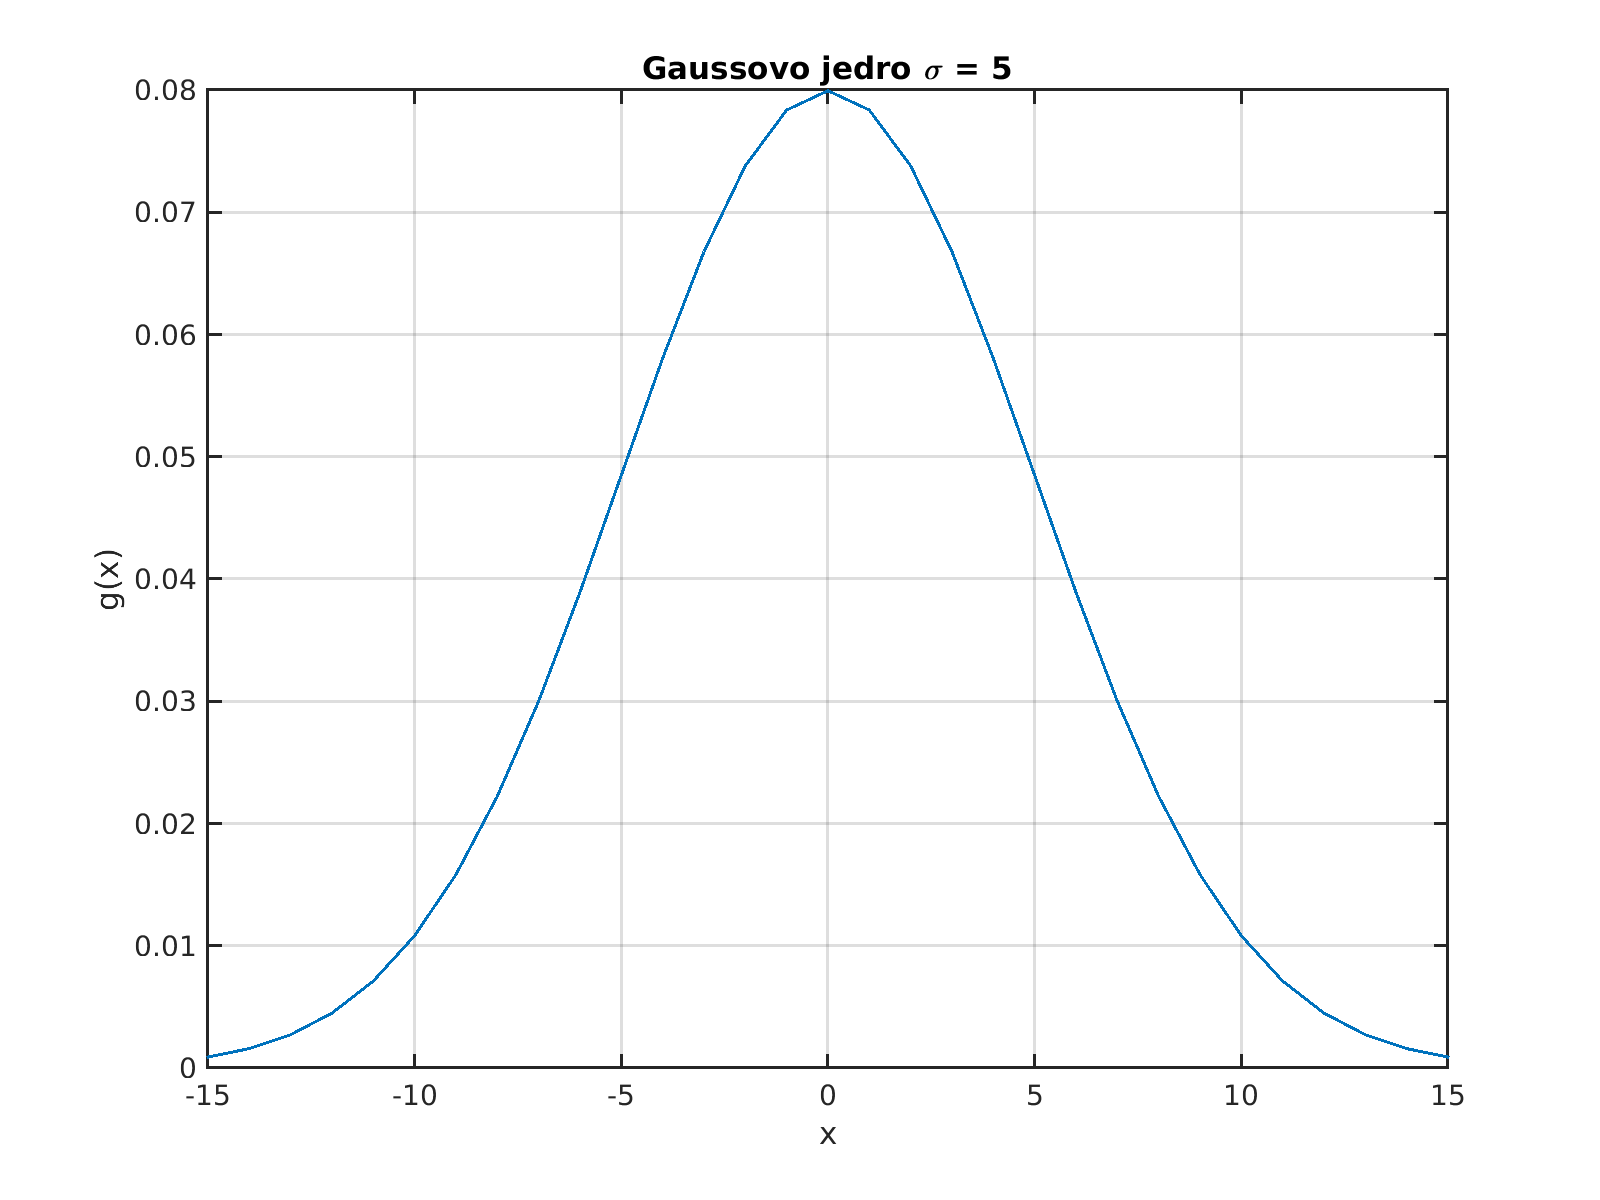
\includegraphics[width=0.7\columnwidth]{./Slike/gauss-kernel.png}
\caption{Gaussovo jedro s standardnim odklonom $\sigma=5$. }
\label{fig:gauss}
\end{figure}


Gaussov filter je vrsta filtra tekočega povprečja, ki je zelo primeren za izločevanje odvečnega šuma \cite{smith1997scientist}. Ker je karakteriziran z impulznim odzivom, ki je simetričen okoli ničelnega vzorca, gre za vrsto filtra z ničelno fazo. To pomeni, da je faza v frekvenčnem prostoru vedno $0$ \cite{smith1997scientist}. Ker imamo pri takih filtrih negativne indekse, ga težje uporabljamo. 

Ponavadi filtre uporabljamo v rekurzivni obliki, saj je računanje hitrejše. Impulzni odziv rekurzivnega filtra ni simetričen, zato ima nelinearno fazo \cite{smith1997scientist}. To pomankljivost lahko odpravimo z uporabo dvosmernega filtriranja.

Pri \textbf{dvosmernem filtriranju} najprej filtriramo iz leve proti desni in nato iz desne proti levi \cite{smith1997scientist}. Dobljena signala združimo in dobimo pravilen rezultat.







\section{Transformacija }
% Za testiranje optičnega toka in deskriptorjev, testiranje njihove robustnosti smo naredili več manipulacij, za boljšo predstavo o delovanju
\begin{equation}
\vec{M}_{int} = \begin{bmatrix}
	f_u & 0 & c_u \\
    0 & f_v & c_v \\
    0 & 0 & 1
\end{bmatrix}
\label{eq:intrinsic}
\end{equation}

\begin{equation}
\vec{R}_\phi = \begin{bmatrix}
\cos(\phi) & - \sin(\phi) & 0 \\
\sin(\phi) & \cos(\phi) & 0 \\
0 & 0 & 1
\end{bmatrix}
\label{eq:roll}
\end{equation}

\begin{equation}
\vec{R}_\theta = \begin{bmatrix}
1 & 0 & 0 \\
0 & \cos(\theta) & - \sin(\theta) \\
0 & \sin(\theta) & \cos(\theta)
\end{bmatrix}
\label{eq:pitch}
\end{equation}

\begin{equation}
\vec{R}_\psi = \begin{bmatrix}
\cos(\psi) & 0 & \sin(\psi) \\
0 & 1 & 0 \\
- \sin(\psi) & 0 & \cos(\psi) 
\end{bmatrix}
\label{eq:yaw}
\end{equation}


\begin{equation}
\vec{R} = \vec{R}_\phi \vec{R}_\theta \vec{R}_\psi
\label{eq:rotation}
\end{equation}


\begin{equation}
\vec{M}_{ext} = \begin{bmatrix}
	\vec{R} & \vdots & \vec{t}
\end{bmatrix}
\label{eq:extrinsic}
\end{equation}


\begin{equation}
\vec{H} = \vec{M}_{int} \vec{M}_{ext}
\label{eq:homography}
\end{equation}


\section{Evaluacijske metrike}
rmse snr mera prekrivanja področja, rae r 



\section{Materiali}
\subsection{Zlati standard}
\subsection{Senzorji v lab}
\subsection{Senzorji na terenu}
\subsection{Sinhornizacija časa}



